\chapter{Kryptologie}
\renewcommand{\chaptertitle}{Kryptologie}

\lehead[]{\sf\hspace*{-2.00cm}\textcolor{white}{\colorbox{lightblue}{\makebox[1.60cm][r]{\thechapter}}}\hspace{0.17cm}\textcolor{lightblue}{\chaptertitle}}
\rohead[]{\textcolor{lightblue}{\chaptertitle}\sf\hspace*{0.17cm}\textcolor{white}{\colorbox{lightblue}{\makebox[1.60cm][l]{\thechapter}}}\hspace{-2.00cm}}
%\chead[]{}
\rehead[]{\textcolor{lightblue}{AvHG, Inf, My}}
\lohead[]{\textcolor{lightblue}{AvHG, Inf, My}}

Die Kryptologie ist die Wissenschaft, die sich mit Verfahren zur Ver- und
Entschlüsselung von Daten beschäftigt. Sie lässt sich unterteilen in die beiden
Bereiche \emph{Kryptografie} und\emph{Kryptoanalyse}. 

Während die Kryptografie sich damit beschäftigt, Verfahren zu entwickeln, die
benutzt werden können, um Nachrichten für andere unlesbar zu machen und es dem legitimen
Empfänger erlauben, die verschlüsselte Nachricht wieder zu entschlüsseln,
beschäftigt sich die Kryptoanalyse mit der Sicherheit (oder anders herum gesagt:
der Angreifbarkeit) von kryptografischen Verfahren.

Ein zentraler Begriff der Kryptologie ist der des \emph{Schlüssels}. Mit Hilfe
des Schlüssels kann die Nachricht auf der Senderseite verschlüsselt und auf der
Empfängerseite auch wieder entschlüsselt werden.

Ohne Kenntnis des Schlüssels ist die verschlüsselte Nachricht nicht oder nur mit
hohem Aufwand (Kryptoanalyse) zu entschlüsseln.

\begin{center}
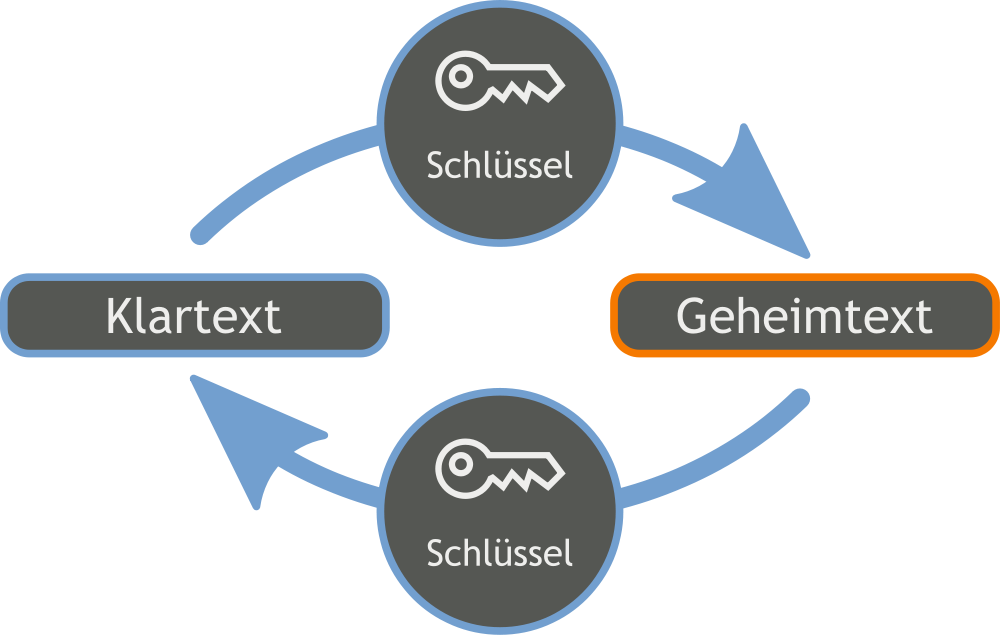
\includegraphics[width=0.6\textwidth]{./inf/SEKII/41_Kryptologie/symmetricCryptography.png}
% http://commons.wikimedia.org/wiki/File:Orange_blue_symmetric_cryptography_de.svg
% Creative Commons CC0 1.0 Universal Public Domain Dedication
\end{center}

Der Klartext wird mittels eines Schlüssels verschlüsselt. Mit Hilfe des selben
Schlüssels kann der Geheimtext wieder entschlüsselt werden

\section{Monoalphabetische Verfahren}

Bei monoalphabetischen Verfahren wird aus einem Klartextbuchstaben immer
derselbe Geheimtextbuchstabe.

\subsection{Das Caesar-Verfahren}

Dieses Verfahren wurde von Julius Caesar 50 Jahre vor Christus benutzt. Das
Alphabet wird dabei einfach um mehrere Buchstaben verschoben. Zum Beispiel um
drei Buchstaben:

\bgroup
\def\arraystretch{1.2}
\setlength{\tabcolsep}{.5em}
\begin{tabular}{|c|c|c|c|c|c|c|c|c|c|c|c|c|c|c|c|c|c|c|c|c|c|c|c|c|c|}\hline
a & b & c & \textbf{d} & \textbf{e} & \textbf{f} & \textbf{g} & \textbf{h} &
\textbf{i} & \textbf{j} & \textbf{k} & \textbf{l} & \textbf{m} & \textbf{n} &
\textbf{o} & \textbf{p} & \textbf{q} & \textbf{r} & \textbf{s} & \textbf{t} &
\textbf{u} & \textbf{v} & \textbf{w} & \textbf{x} & \textbf{y} & \textbf{z}
\\ \hline
\textbf{D} & \textbf{E} & \textbf{F} & \textbf{G} & \textbf{H} & \textbf{I} &
\textbf{J} & \textbf{K} & \textbf{L} & \textbf{M} & \textbf{N} & \textbf{O} &
\textbf{P} & \textbf{Q} & \textbf{R} & \textbf{S} & \textbf{T} & \textbf{U} &
\textbf{V} & \textbf{W} & \textbf{X} & \textbf{Y} & \textbf{Z} & A & B & C
\\ \hline
\end{tabular}
\egroup

Damit wird aus dem Klartext \myUserInput{hallo} der Geheimtext
\myUserInput{KDOOR}.

\subsubsection{Kryptoanalyse des Caesar-Verfahrens}

Das Caesar-Verfahren ist schon über 2000 Jahre alt. Es ist deshalb nicht
erstaunlich, dass es sehr leicht zu brechen ist. Die Analysemethode nennt sich
\emph{Brute-Force}, was nichts anderes heißt als \glqq rohe Gewalt\grqq . Der
Trick besteht darin, dass einfach alle möglichen Schlüssel ausprobiert werden,
und man schaut, was dabei jeweils als Klartext herauskommt.


\subsection{Substitutionsverfahren}

Irgendwann haben Caesars Nachfahren herausgefunden, dass dieses Verfahren nicht
sehr sicher ist. Wenn jedoch die Anzahl der möglichen Schlüssel erhöht werden
könnte, dann würde die Kryptoanalyse massiv erschwert werden. Dies gelingt mit
dem Substitutionsverfahren. Dabei wird jeder Buchstabe des Klartextes durch
einen beliebigen Buchstaben aus dem Geheimtext ersetzt (\glqq
substituieren\grqq\ = \glqq ersetzen\grqq ). Es werden nicht mehr alle
Buchstaben um gleich viele Stellen verschoben wie beim Caesar-Verfahren.
Damit man sich dazu den Schlüssel gut merken kann, geht man folgendermaßen
vor:

Die Buchstaben des Klartextalphabets werden der Reihe nach hingeschrieben.
Darunter wird zuerst das Schlüsselwort (im Beispiel: \myUserInput{KRYPTO})
geschrieben, und dann kommen der Reihe nach alle im Schlüsselwort nicht
benutzten Buchstaben des Alphabets.

Beispiel mit Schlüsselwort \myUserInput{KRYPTO}:	

\bgroup
\def\arraystretch{1.2}
\setlength{\tabcolsep}{.5em}
\begin{tabular}{|c|c|c|c|c|c|c|c|c|c|c|c|c|c|c|c|c|c|c|c|c|c|c|c|c|c|}\hline
a & b & c & d & e & f & g & h & i & j & k & l & m & n & o & p & q & r & s
& t & u & v & w & x & y & z \\ \hline
\textbf{K} & \textbf{R} & \textbf{Y} & \textbf{P} & \textbf{T} & \textbf{O} & A
& B & C & D & E & F & G & H & I & J & L & M & N & Q & S & U & V & W & X & Z \\
\hline
\end{tabular}
\egroup

Damit wird aus dem Klartext \myUserInput{hallo} der Geheimtext
\myUserInput{BKFFI}.


\section{Polyalphabetische Verschlüsselungsverfahren}

Nachdem die Kryptoanalytiker auch das Substitutionsverfahren geknackt hatten,
waren die Verschlüsselungsspezialisten wieder gefragt. Solange aus einem
Klartextbuchstaben immer der gleiche Geheimtextbuchstabe entsteht, kann man
immer die Häufigkeitsanalyse anwenden.

So entstand die polyalphabetische Verschlüsselung, bei der aus einem
Klartextbuchstaben nicht immer der gleiche Geheimtextbuchstabe wird (\glqq
poly\grqq\ = \glqq viel\grqq ).

\subsection{Vigenère-Verfahren}

Das bekannteste polyalphabetische Verschlüsselungsverfahren heißt Vigenère und
funktioniert folgendermaßen:

\bgroup
\def\arraystretch{1.2}
\setlength{\tabcolsep}{.5em}
\begin{tabular}{cccccccccccccccccccc}
  & & d & i & e & s & i & s & t & d & e & r & k & l & a & r & t & e & x & t \\
+ & & \textbf{k} & \textbf{e} & \textbf{y} & k & e & y & k & e & y & k & e & y &
k & e & y & k & e & y
\\
\hline
  & & O & N & D & D & N & R & E & I & D & C & P & K & L & W & S & P & C & S \\
\end{tabular}
\egroup   
   
Der Schlüssel (hier \myUserInput{key}) wird endlos wiederholt unter den Klartext
geschrieben. Danach werden zu den Buchstaben des Klartextes die Buchstaben des
Schlüssels hinzu addiert. So wird aus \myUserInput{d} (4.~Buchstabe) plus
\myUserInput{k} (11.~Buchstabe) ein \myUserInput{O} (4 + 11 = 15.~Buchstabe).
Eine verschlüsselte Nachricht wird entschlüsselt, indem der Schlüssel vom
Geheimtext subtrahiert wird.

\subsubsection{Kryptoanalyse des Vigenère-Verfahren}

Wieso ist das Knacken der Nachricht auch bei einer polyalphabetischen
Verschlüsselung noch möglich? Der Schlüssel hat eine bestimmte Länge, zum
Beispiel 3 wie im oben gewählten Beispiel.

Das hat zur Folge, dass jeder dritte Buchstabe um die gleiche Anzahl Buchstaben
verschoben wird (der erste, der vierte, etc., alle werden um k = 11 Stellen
verschoben).

Wenn nun wie im Beispiel an der zweiten und fünften Stelle der gleiche Buchstabe
steht (\myUserInput{i}) so wird aus diesem auch der gleiche Geheimtextbuchstabe
(\myUserInput{N}):

\bgroup
\def\arraystretch{1.2}
\setlength{\tabcolsep}{.5em}
\begin{tabular}{cccccccccccccccccccc}
  & & d & \textbf{i} & e & s & \textbf{i} & s & t & d & e & r & k & l & a & r &
  \textbf{t} & e & x & \textbf{t}
  \\
+ & & k & \textbf{e} & y & k & \textbf{e} & y & k & e & y & k & e & y &
k & e & \textbf{y} & k & e & \textbf{y}
\\
\hline
  & & O & \textbf{N} & D & D & \textbf{N} & R & E & I & D & C & P & K & L & W &
  \textbf{S} & P & C & \textbf{S}
  \\
\end{tabular}
\egroup

Durch solche auftretende Muster lässt sich per Computer relativ einfach die
Schlüssellänge L bestimmen, indem man gleiche Buchstabenfolgen im Geheimtext
sucht und deren Abstand bestimmt. Hat man erst einmal die Schlüssellänge L
nimmt man zur Bestimmung des 1.~Buchstabens des Schlüssels den 1., den 1+L, den
1+2L usw.\ Buchstaben und macht auf diesen eine einfache Häufigkeitsanalyse.
Dies funktioniert, da alle diese Buchstaben um die gleiche Anzahl Stellen
verschoben wurden (wie beim Caesar-Verfahren). Man muss nur den häufigsten
Buchstaben finden, und schon ist die Verschiebung bekannt (durch Vergleich mit
'e').

\subsection{One-Time-Pad}

Das Knacken von Vigenère gelingt, da es wegen der fixen Schlüssellänge zu
Wiederholungen kommt. Nimmt man einen Schlüssel der mindestens genau so lang ist
wie der zu verschlüsselnde Text gibt es keine Wiederholungen. Dieses Verfahren
heißt \emph{One-Time-Pad}.

Das One-Time-Pad ist ein 100\% sicheres Verfahren, denn jeder Schlüsselbuchstabe
wird nur ein mal (one time) verwendet. Es hat nur einen -- im wahrsten Sinne des
Wortes großen -- Nachteil: Im vornherein muss ein riesengroßer geheimer
Schlüssel vereinbart werden. Dieses Verfahren wurde während des Kalten Krieges
zwischen Moskau und Washington eingesetzt (\glqq heißer Draht\grqq ). Dafür
mussten regelmäßig Diplomaten mit Koffern voller Zufallszahlen hin und
her reisen.

Denn auch beim One-Time-Pad gilt:

\begin{compactitem}
\item Der Schlüssel muss über einen sicheren separaten Kanal übermittelt werden.
\item Ist der Schlüssel dem Gegner bekannt ist die Sicherheit dahin.
\end{compactitem}

\subsection{DES}

Das heute im kommerziellen Gebrauch am häufigsten eingesetzte Verfahren heißt
\emph{DES} (\glqq Data Encryption Standard\grqq ). Es funktioniert im Prinzip
wie ein mehrfach hintereinander angewandtes Substitutionsverfahren.

Der DES erlaubt mit 56 Bits Schlüssellänge = 72 057 594 037 927 936 = 72
Billiarden mögliche Schlüssel. Dennoch ist dies heute nicht mehr ausreichend:
DES kann in wenigen Stunden mittels der Brute-Force-Methode geknackt werden!

\subsection{IDEA}

Der \emph{IDEA} (\glqq International Data Encryption Algorithm\grqq )
funktioniert ähnlich wie DES und arbeitet mit 128 Bits Schlüssellänge. Damit
besitzt er $2^{128}$ = $3.43669 \cdot 10^{38}$ mögliche Schlüssel. Dies zu
knacken benötigt derzeit viele Jahre. Deshalb gilt der IDEA heute als
sicher.


\section{Asymmetrische Verschlüsselung}

Bei symmetrischen Verschlüsselungsverfahren, bei denen zum Kodieren und
Dekodieren derselbe Schlüssel verwendet wird, besteht das Problem, dass der
Empfänger der Nachricht irgendwie auf einem geheimen Kanal an den Schlüssel
kommen muss. Wenn die Übertragung des Schlüssels abgefangen wird, kann die
Nachricht auch von Fremden entschlüsselt werden. Dieses Problem wird mit der
asymmetrischen Verschlüsselung gelöst.

\subsubsection{Grundprinzip}

In asymmetrischen Verschlüsselungsverfahren existieren zwei verschiedene
Schlüssel, von denen einer zur Verschlüsselung und der andere zur
Entschlüsselung verwendet wird. Beide Schlüssel sind mathematisch miteinander
verbunden. Das zusammengehörende Schlüsselpaar besteht aus:

\begin{compactitem}
\item[\textbf{Private Key}] Dieser verbleibt grundsätzlich beim Eigentümer des
Schlüssels.
\item[\textbf{Public Key}] Dieser ist öffentlich bekannt und kann von jedermann
benutzt werden.
\end{compactitem}

\subsubsection{Anwendungen}

Verschlüsselung: Eine Nachricht wird mit dem Public Key des Empfängers
verschlüsselt. Sie kann dann nur mit Hilfe des zugehörigen Private Keys
entschlüsselt werden. Deshalb kann niemand anders als der Empfänger die
Nachricht dekodieren.

Digitale Unterschriften: Für den öffentlich lesbaren Text wird eine Prüfsumme
berechnet. Die Prüfsumme wird mit dem Private Key des Senders kodiert. Mit dem
bekannten Public Key des Senders kann nun jedermann die Prüfsumme dekodieren
und so überprüfen, ob die Nachricht tatsächlich von der angegebenen Person
stammt. Diese digitalen Unterschriften gelten als unfälschbar und sind seit
Januar 2000 im deutschen Signaturgesetz rechtlich der handschriftlichen
Unterschrift gleichgestellt.

\subsubsection{Mathematische Grundlage}

Zum Verschlüsseln werden mathematische Einweg-Operationen angewandt, deren
Umkehrung erheblich komplizierter ist, als die Operation selbst. Das Produkt
zweier großer Primzahlen zu berechnen ist auch von Hand nicht besonders schwer.
Ein Algorithmus, der eine gegebene (sehr große) Zahl in ihre Primfaktoren
zerlegt, ist dagegen viel langwieriger. Es ist bisher kein effektives Verfahren
dafür bekannt. Die Grundideen zur Verwendung mathematischer Einweg-Funktionen
stammen möglicherweise aus den Sechziger Jahren (Communications Electronics
Security Group), wurden aber durch die Veröffentlichungen von Whitefield Diffie
und Martin Hellman im Jahre 1976 bekannt. Auf dieser Basis wurde 1978 ein auf
Potenzierung und ganzzahliger Division mit Rest (Modulo-Operation) beruhendes
Verfahren vorgestellt. Die Entwickler Ron Rivest, Adi Shamir und Leonard
Adleman vermarkten dieses Verfahren weltweit unter dem Namen \emph{RSA}. Für
Privatpersonen ist die Nutzung des RSA-Algorithmus mit dem Programm \emph{Pretty
Good Privacy} (PGP) kostenlos. Das Verfahren ermittelt für jeden Teilnehmer
einen privaten und einen öffentlichen Schlüssel. Dazu werden zunächst per
Zufall zwei üblicherweise 1024 Bit lange Primzahlen $p$ und $q$ ausgewählt.

\subsection{RSA-Algorithmus}

Zuerst werden per Zufall zwei große Primzahlen $p$ und $q$ erzeugt, die später
vernichtet werden. Aus den Primzahlen berechnet man die Zahlen

\begin{eqnarray*}
n &=& p \cdot q\\
s &=& (q - 1) \cdot (p - 1)
\end{eqnarray*}

\subsubsection{Öffentlicher Schlüssel}

Für den  Public Key wird eine Zahl $e$ so gewählt, dass $e$ und $s$ keinen
anderen gemeinsamen Teiler besitzen als die Zahl 1. $e$ muss dabei kleiner
sein als $s$.

\subsubsection{Privater Schlüssel}

Für den Private Key wird eine Zahl $d$ so gewählt, dass $(d \cdot e) \bmod s$
den Wert 1 ergibt. ($\bmod$ ist der Modulo-Operator, der in Java als
\lstinline|%| geschrieben wird)

\subsubsection{Verschlüsselung einer Botschaft}

Die Botschaft wird zunächst in Zahlen umgewandelt. Die Zahlen werden blockweise
kodiert, wobei jeder Block kleiner als $n$ sein muss. Ein in Zahlen kodierter
Klartext $b$ wird folgendermaßen in einen Geheimtext $c$ kodiert:

\[
c = b^e \bmod n
\]

\subsubsection{Entschlüsseln einer Botschaft}

Ein Geheimtext $c$ wird folgendermaßen in den Klartext $b$ zurück gewandelt:

\[
b = c^d \bmod n
\] 

\subsubsection{Schwachstelle des Public Key Verfahrens}
	
Ein Angriffspunkt ist die Verbreitung des öffentlichen Schlüssels. Man kann
seinen öffentlichen Schlüssel in einer Datei speichern, die man dann an seine
Freunde weitergeben oder im Internet veröffentlichen kann. Was aber, wenn ein
Fremder einen öffentlichen Schlüssel unter deinem Namen veröffentlicht? Eine mit
diesem Schlüssel chiffrierte Nachricht kann dann nur von dem Fremden gelesen
werden und nicht von dir selbst.\footnote{Quelle: Sicherheit in Netzen --
Netzmafia \url{http://www.netzmafia.de/skripten/sicherheit/sicher5.html}}


\section{Anwendungsgebiete der Kryptographie}

Kryptographische Methoden wurden und werden an vielen Stellen und in vielen
Anwendungsszenarien eingesetzt.

\begin{compactitem}
\item Signierung von e-Mails (Nachweis der Authentizität der Nachricht).	

\url{http://de.wikipedia.org/wiki/E-Mail-Verschlüsselung}
\item Verschlüsselung von Datenverkehr über unsichere Verbindungen (etwa
Online-Banking). Dazu gibt es eine ganze Reihe von Protokollen. Beispiele:
HTTPS statt HTTP, IMAPS statt IMAP oder auch die komplette Kapselung von
Netzwerkverkehr über VPNs (Virtual Private Networks), womit beispielsweise
verschiedene Standorte eines Unternehmens über das Internet (unsicher) so
verbunden werden können, dass die vertraulichen Inhalte des internen
Firmennetzwerkes durch \glqq Mithörer\grqq\ nicht entschlüsselt werden können.

\url{http://de.wikipedia.org/wiki/Transport_Layer_Security}

\url{http://de.wikipedia.org/wiki/Virtual_Private_Network}

\item Verschlüsselung von Funkverkehr (etwa Mobilfunknetze).	 

\url{http://de.wikipedia.org/wiki/Global_System_for_Mobile_Communications#Sicherheitsfunktionen}
\item Rechtssicherer elektronischer Geschäftsverkehr. Etwa bei
Vertragsabschlüssen.

\url{http://de.wikipedia.org/wiki/Signaturgesetz_(Deutschland)}
\item Geldautomaten übertragen die PIN nie unverschlüsselt:	

\url{http://de.wikipedia.org/wiki/Encrypting_PIN_Pad}
\item Der Netzwerkverkehr in WLANs kann (und wird meistens auch) verschlüsselt
um den naturgemäß offenen Zugang zu beschränken:

\url{http://de.wikipedia.org/wiki/Wlan#Datensicherheit}
\item PayTV: Hier wird der \glqq Content\grqq\ (also das Fernsehsignal) so
verschlüsselt, dass nur der zahlende Kunde das Programm richtig sehen kann. Für
alle anderen gibt es nur Bildrauschen.

\url{http://de.wikipedia.org/wiki/Zugangsberechtigungssystem}
\item Kryptowährungen wie etwa Bitcoins als virtuelle Zahlungsmittel existieren
nicht als Münzen oder Geldscheine, sondern lediglich als Dateien. Diese müssen
entsprechend stark kryptographisch gesichert sein.

\url{http://de.wikipedia.org/wiki/Kryptowährung}
\end{compactitem}


\section{Kryptoanalyse}

Die Kryptoanalyse beschäftigt sich mit der Sicherheit aber auch den
Schwachstellen von kryptographischen Verfahren. Es folgt eine Auflistung der
gängigsten Angriffsmethoden gegen kryptographische Verfahren, mit dem Ziel die
Verschlüsselung zu knacken:

\begin{compactitem}
\item[\textbf{Brute Force}] Typischerweise mit Hilfe von Computern werden
\glqq einfach\grqq\ alle möglichen Schlüssel durchprobiert. Das wird umso
aufwändiger (im zu wünschenden Extremfall aussichtslos), je größer die Anzahl
der möglichen Schlüssel ist. Eng damit verknüpft ist die sogenannte
Schlüssellänge: Je länger ein Schlüssel, desto größer ist der sogenannte
\glqq Schlüsselraum\grqq\ der durchsucht werden muss.

\url{http://de.wikipedia.org/wiki/Brute_force#Kryptologie}

\item[\textbf{Häuffigkeitsanalyse}] Im speziellen (aber nicht ausschließlich)
bei monoalphabetischen Verfahren kann man über die statistische Analyse des
verschlüsselten Textes Rückschlüsse auf die Verschlüsselung ziehen. So ist etwa
in der deutschen Sprache das 'E' der häufigste Buchstabe. Ein hinreichend
langer deutscher Text wird deshalb auch in seiner verschlüsselten Form schnell
zeigen, welches Zeichen dem 'E' entspricht.

\url{http://de.wikipedia.org/wiki/Häufigkeitsanalyse}

\item[\textbf{Social Engineering}] Über den direkten Kontakt mit der
\glqq Zielperson\grqq\ (oder Personen aus deren Umfeld) können oft Informationen
gewonnen werden, die entweder direkt (\glqq Hallo, ich arbeite bei der Bank, bei
der Sie Online-Banking betreiben. Jemand hat versucht sich in Ihr Konto zu
hacken. Ich muss Sie deshalb bitten, mir Ihr Passwort und die nächsten TANs zu
nennen.\grqq ), oder indirekt (Informationen, die anschließend zum Erraten von
Schlüsseln bzw. Passwörtern genutzt werden können).

\url{http://de.wikipedia.org/wiki/Social_Engineering_(Sicherheit)}

\item[\textbf{Erraten}] Schlechte Passwörter lassen sich erraten (Name eines
Verwandten oder Haustieres, Geburtstage oder ähnliches. Oft in Verbindung mit
\glqq Social Engineering\grqq .

\item[\textbf{Wörterbuchangriffe (Dictionary Attacks)}] Eine übliche
rechnergestützte Methode um schlechte/schwache Passwörter zu knacken. Dabei
werden von einem Rechner alle möglichen bekannten Wörter (auch Namen und
Geburtstage) aus einer Wörterbuch-Datei, oft auch kombiniert mit zusätzlichen
Ziffern oder der inzwischen üblichen Ersetzungen wie etwa '3' für 'E' etc.

\url{http://de.wikipedia.org/wiki/Dictionary_Attack}
\end{compactitem}

